\section{Design}

\subsection{Barrel layout and support structure}

The SVT comprises 21504 channels of wire-bonded triplets of p-on-n AC-coupled single-sided silicon micro-strip sensors in six layers (three concentric polygonal regions that have 10, 14, and 18 double-sided modules positioned at radii of 65, 93, and 120 mm). The SVT is enclosed by a Faraday cage with an inner radius of 57 mm (with 6 mm clearance to the inner shell of the target scattering chamber) and an outer radius of 133 mm. To minimize multiple scattering, a unique module design with extra long 33~cm strips has been developed to reduce the material budget to about 1.4$\%$ of a radiation length per region (two silicon planes) for normal incidence tracks, which is essential for tracking at low momenta~\cite{Vertex2016}. The module dimensions are 41.9 cm $\times$ 4.2 cm $\times$ 0.39 cm. All of the SVT modules are identical to minimize production costs. There are no overlaps of adjacent modules and minimal clearance between them to satisfy material budget and acceptance constrains.

\begin{figure}[hbt] 
\centering 
\includegraphics[width=1.0\columnwidth,keepaspectratio]{barrel-faradaycage.png}
\caption{Layout of the barrel and the Faraday Cage. Copper supports are shown in yellow.  Supports are bolted directly to the cold plate. The silicon sensors are shown in green.}
\label{fig:barrel-faradaycage}
\end{figure}

%\begin{wrapfigure}{l}{0.5\columnwidth}
%\centering 
%\includegraphics[width=1.0\columnwidth]{cvt-crosssection.png}
%\caption{CVT crossection.}
%\label{fig:cvt-crosssection}
%\end{wrapfigure}

%Figure~\ref{fig:cvt-crosssection} shows the side view of the detector. 

The modules  are mounted between upstream and downstream rings (see Fig.~\ref{fig:barrel-faradaycage}). For each region the upstream ring is attached to the cold plate with screws. The upstream support ring provides a mounting surface for the modules on the upstream end of the detector. It also provides a conduction path for heat to be transferred from the modules to the coolant flowing through the cold plate. 

\begin{figure}[hbt] 
\centering 
\includegraphics[width=0.8\columnwidth,keepaspectratio]{upstreamring.png}
\caption{Upstream support ring attached to the cold plate.}
\label{fig:upstreamring}
\end{figure}

 The SVT modules are cantilevered off a chilled cold plate, designed to provide mechanical support and to remove heat generated by the electronics, located at the upstream end of the module outside of the tracking volume (see Fig.~\ref{fig:upstreamring}). The cold plate is bolted to the mounting tube that is attached to the insertion cart with the support tube. 
 
The cold plate and upstream ring are attached to the mounting tube. The mounting surfaces of the upstream and downstream rings are machined closely coupled in a single step to guarantee planarity. The rings of each region are independent from each other to prevent over-constraining the assembly. This design allows an entire region to be removed as a unit, rather than module by module. The modules in the vertical and near vertical positions provide stiffness to the downstream ring and to a region as a whole. The regions are shifted along the beam axis to match the required angular coverage. The downstream support rings are made from PolyEther Ether Ketone (PEEK)~\cite{NIMVCC}. 

\begin{figure}[hbt] 
\centering 
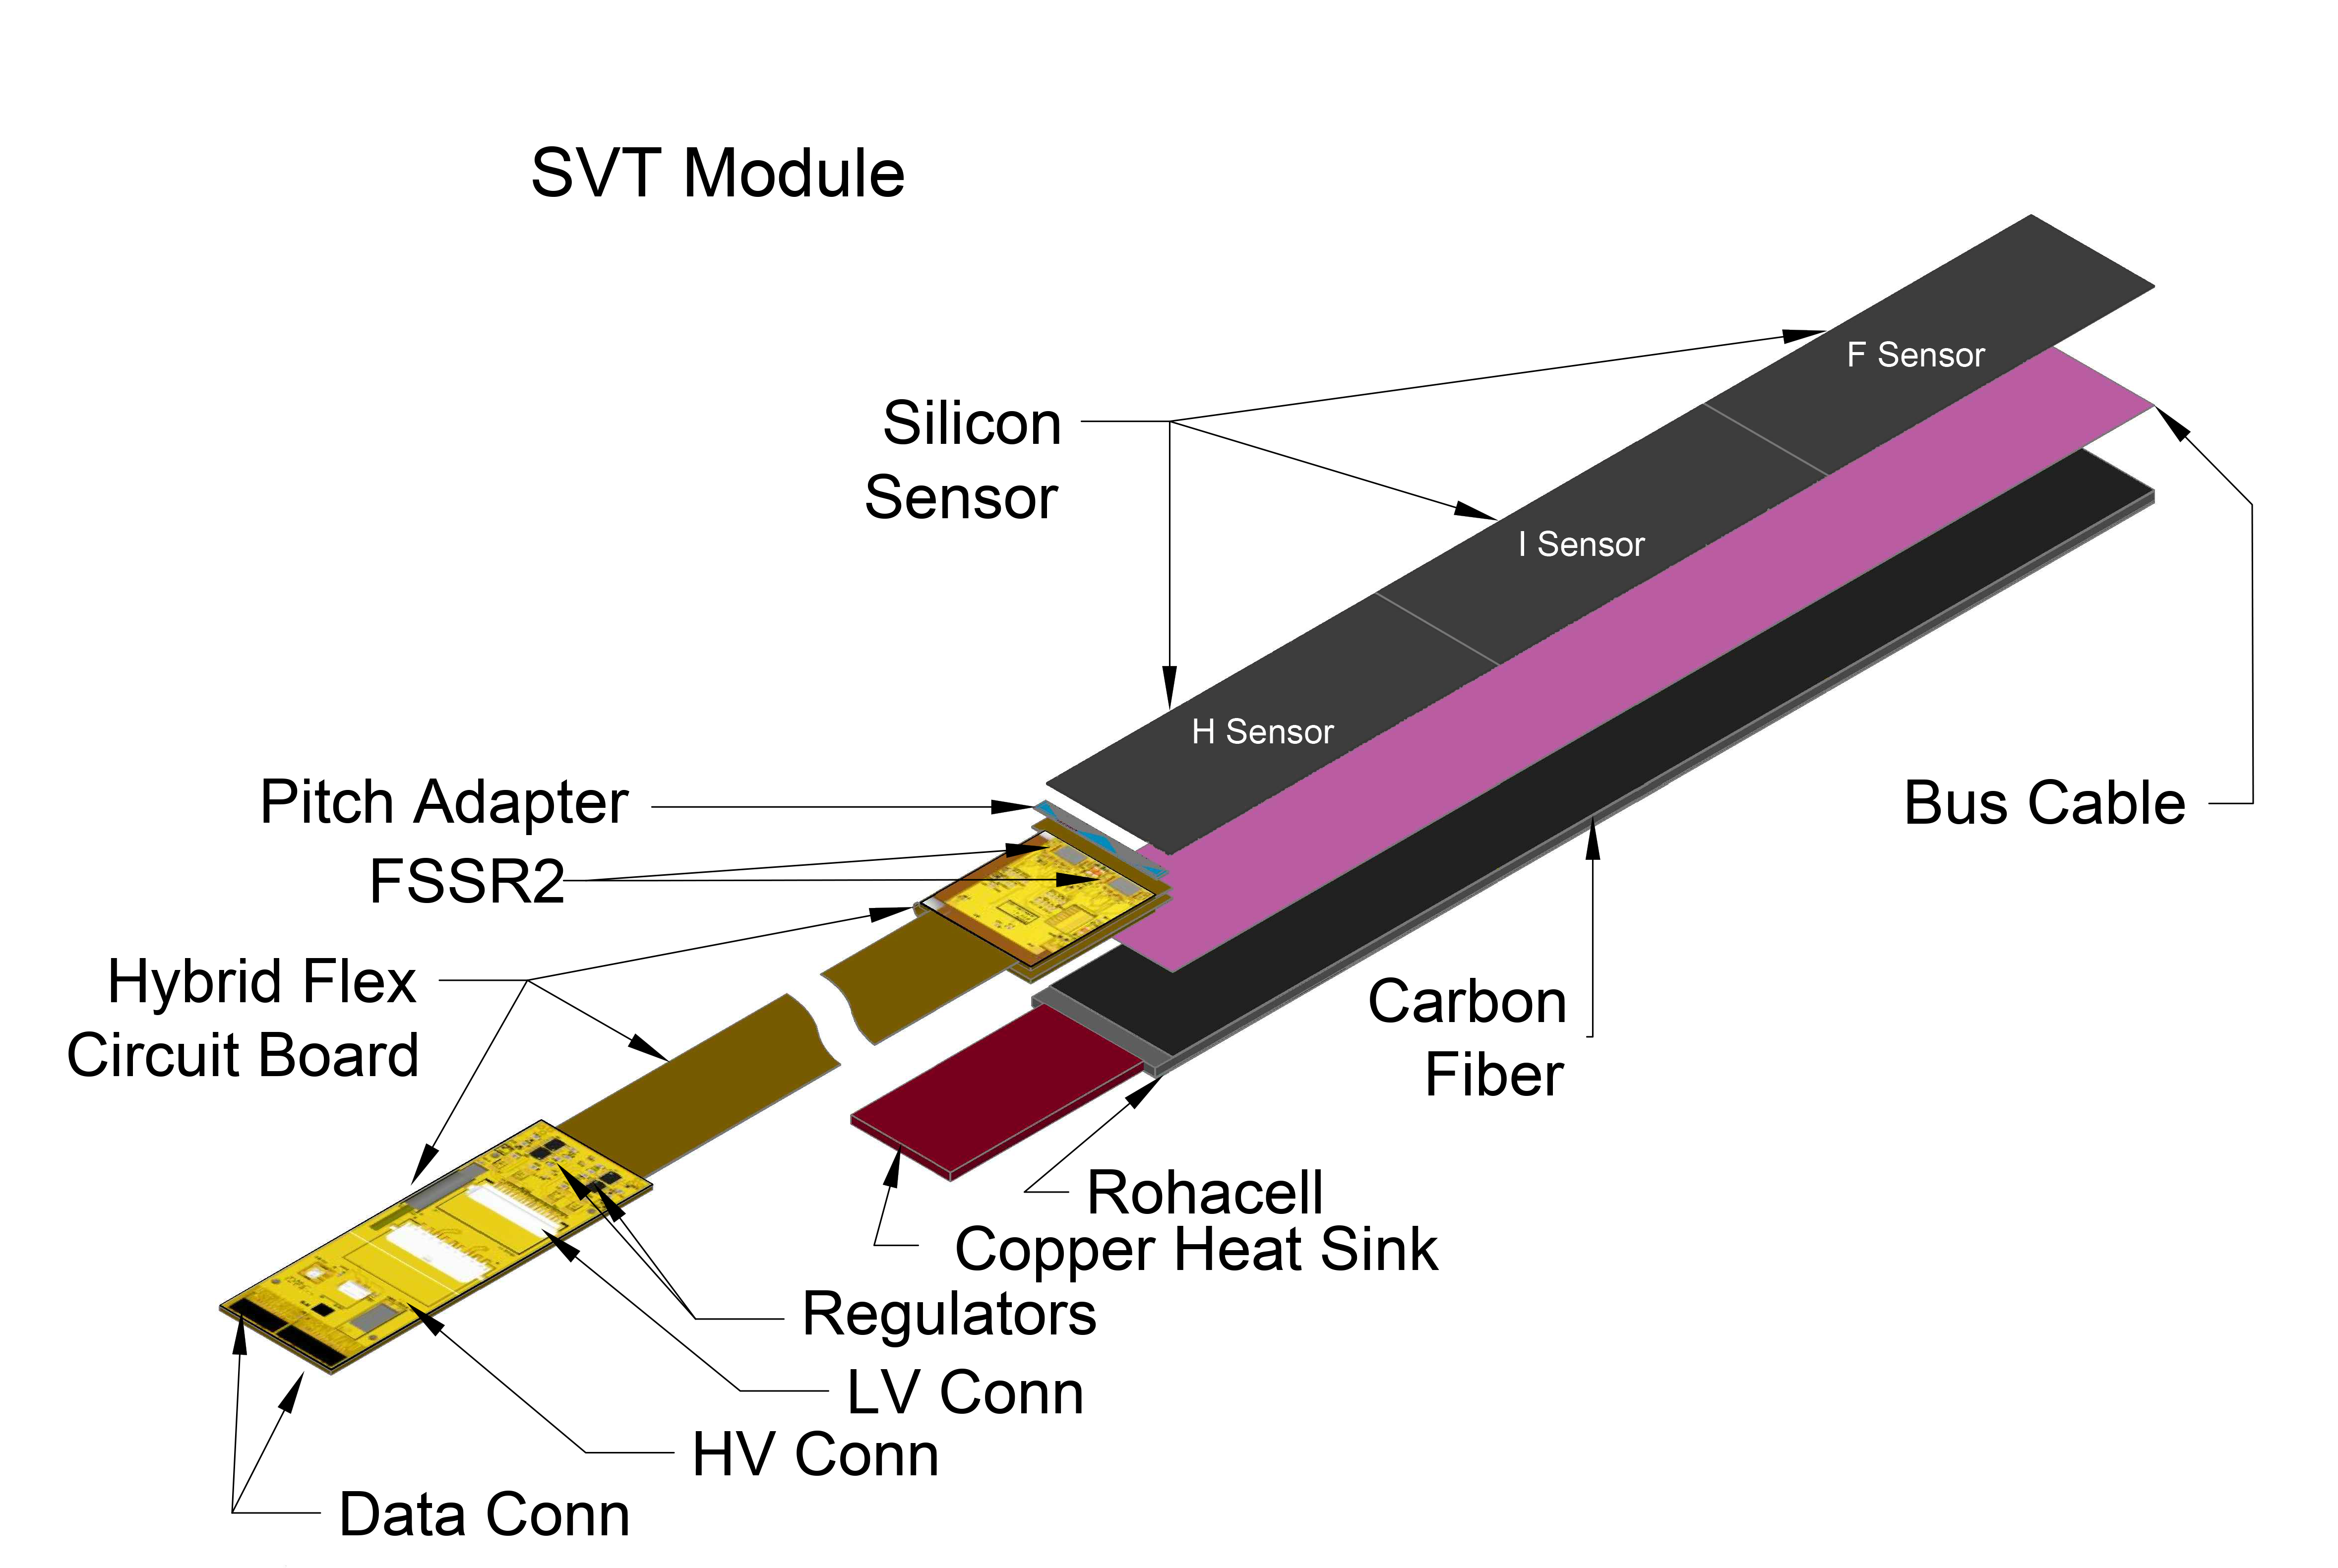
\includegraphics[width=1.0\columnwidth,keepaspectratio]{module.png}
\caption{Layout of an SVT module.}
\label{fig:module}
\end{figure}

\subsection{Module design}

The SVT uses single-sided 320-$\mu$m thick microstrip sensors fabricated by Hamamatsu, mounted on each side of the module (see Fig.~\ref{fig:module}). All modules have 3 types of sensors: H (Hybrid), I (Intermediate), and F (Far). The sensors were cut from 6 inch wafers with resistivity of 5 $\kiloohm$ and <100> surface orientation, with 2 sensors per wafer to maximize the yield. All sensors have the same size, 112$\times$42 mm. There are three daisy-chained sensors per layer (six per module) with a 110~$\mu$m gap between them. 

\begin{figure}[hbt] 
\centering 
\includegraphics[width=1.0\columnwidth,keepaspectratio]{strip-layout.png}
\caption{Sensor strip layout.}
\label{fig:strip-layout}
\end{figure}

Each layer has 256 strips with linearly varying angles of 0$^\circ$--3$^\circ$ (constant $\phi$ pitch of 1/85$^\circ$) to minimize the dead sensor area. The first readout strip is parallel to the longitudinal axis of the module; the last readout strip has an angle of 3$^\circ$ with respect to this axis (see Fig.~\ref{fig:strip-layout}). Because of the constant $\phi$ pitch, the lengths of the readout strips of the modules vary from 0.5 cm to 33 cm. At the hybrid side, the intermediate strip pitch is 78 $\mu$m and the readout pitch is 156 $\mu$m. The strip-to-pitch ratio is 0.256 for all three types of sensors. Fig.~\ref{fig:sensor} shows the cross-sectional view of the sensor. The aluminum strip width is 26 $\mu$m and is AC-coupled via the SiO$_2$ layer to the 20-$\mu$m wide $p$+ implant strips, which are ~1.2 $\mu$m below the aluminum strips. The total strip capacitance at 1 MHz is below 1.3 pf/cm and coupling capacitance above 10 pf/cm. The implant strips are grounded via 1.5~$\megaohm$ polysilicon resistors. The unpassivated aluminum backplane (ohmic contact) is connected to the positive side of the power supply; the $n$-bulk volume of the sensor is depleted via the highly doped $n$++ layer. The guard ring is surrounding the sensitive area to reduce the surface currents from the edges of the detector. The 42-mm width of the sensor accommodates 256 readout strips and the ~1 mm keep-out zones along the edge of the sensor.

\begin{figure}[hbt] 
\centering 
\includegraphics[width=1.0\columnwidth,keepaspectratio]{sensor.png}
\caption{Cross-sectional view of a sensor showing the different layers and the spacing of the strips (the dimension units are in $\mu$m).}
\label{fig:sensor}
\end{figure}

\begin{figure}[hbt] 
\centering 
\includegraphics[width=1.0\columnwidth,keepaspectratio]{backing-structure.png}
\caption{The module backing structure.}
\label{fig:backing-structure}
\end{figure}

The sensors are mounted on a backing structure composed of Rohacell 71 core, bus cable, and carbon fiber (see Fig.~\ref{fig:backing-structure}). The carbon fiber skin is made from Mitsubishi type K13C2U fibers oriented in a quasi-isotropic (45/-45/0) pattern. To ensure adequate electrical conductivity, it is co-cured with the bus cable, made from a Kapton sheet with 3-$\mu$m thick and 0.5-mm wide copper traces; one side provides high voltage (HV) to the sensors, a 6$\times$6~mm copper mesh on the other side grounds the carbon fiber.  The Rohacell core under the hybrid board is replaced by a copper heat sink to remove $\sim$2~W of heat generated by the ASIC preamplifier chips. At the downstream end of the module, the Rohacell core is replaced by a PEEK insert. The cross-section of the active area of the module is shown in Fig.~\ref{fig:svt-module-layers}. 

\begin{figure}[hbt] 
\centering 
\includegraphics[width=1.0\columnwidth,keepaspectratio]{svt-module-layers.png}
\caption{The cross-section of the module. The dimensions are in mm.}
\label{fig:svt-module-layers}
\end{figure}

\begin{figure}[hbt] 
\centering 
\includegraphics[width=1.0\columnwidth,keepaspectratio]{pitch-adapter.png}
\caption{One end of the pitch adapter mask, showing the alignment fiducials, wire bonding pads, and traces.}
\label{fig:pitch-adapter}
\end{figure}

A pitch adapter matches the 156~$\mu$m sensor readout pitch to the 50~$\mu$m FSSR2 bonding pad pitch. The pitch adapter~\cite{PA} is a glass plate 41.5$\times$4 mm (tolerance of 50~$\mu$m), with metal traces made of aluminum and copper alloy. The alloy improves electromigration hardness and bonding. The metal layer is sputter deposited. The passivation silicon oxide layer protects the soft aluminum traces from damage. There are two fiducials on the pitch adapter edge next to the sensor and three on the edge next to the hybrid to facilitate alignment. No more than one open trace or two short-circuited traces are allowed per pitch adapter. A section of the pitch adapter is shown in Fig.~\ref{fig:pitch-adapter}. 

\begin{figure}[hbt] 
\centering 
\includegraphics[width=1.0\columnwidth]{HFCB.png}
\caption{Hybrid Flex Circuit Board (HFCB). The level one connect board (left side) is connected to the hybrid area (right side).}
\label{fig:HFCB}
\end{figure}

Both sides of a module are instrumented with a readout system by a single rigid-flex Hybrid Flex Circuit Board (HFCB) located on the upstream end of the module (see Fig.~\ref{fig:HFCB}). The HFCB provides bias to the silicon sensors, and power and control lines to four FSSR2 ASICs located at the edge of the hybrid, two on the top and two on the bottom side. The ASICs are glued to pads on their substrates with conductive epoxy. These pads are the reference for the analog return for the chips. The hybrid area of each HFCB (42 x 82 mm) consists of two rigid boards (top and bottom hybrids) connected by a 10~mm-long wing flex High Density Interconnect (HDI) cable wrapped around the backing structure (see Fig.~\ref{fig:hfcb-wrap}). Both hybrids connect to the module electrically using micro-bonding technology for the signals and bias return, and solder connection for the detector bias and module support ground. The sensors, the pitch adapters, and the HFCB are glued to both sides of the backing structure. 

\begin{figure}[hbt] 
\centering 
\includegraphics[width=1.0\columnwidth,keepaspectratio]{hfcb-wrap.png}
\caption{The wrapping of the HFCB from the top to the bottom silicon layers.}
\label{fig:hfcb-wrap}
\end{figure}

Module services are provided via the level one connect (L1C) board (125 x 41 mm) coupled to the hybrid area via the upstream flex HDI cable (245 mm). The upstream flex HDI cable is routed through 10~mm radial slots in the cold plate. The L1C board hosts two high density Nanonics connectors for data and control lines, Molex Micro-Fit 9-pin connector for high voltage ($\sim$85~V) bias to the sensors, AMP Mini CT 17 pin connector for low voltage (2.5~V) power to the ASICs, hybrid temperature connector, external pulser connector, and four voltage regulators. The L1C board is mounted to the support tube on its own support structure designed to keep each L1C board positioned in line with its module.

The HFCB layer stack up consists of six layers of flexible polyimide sandwiched between two triple layers of rigid FR4 (Flame Retardant glass-reinforced epoxy laminate material). The stack up varies from section to section, the flexible sections (wing and upstream flex) only contain the polyimide, whereas the rigid areas contain all 12 layers. This variation in stack up provides the ability to instrument both the top and bottom sides of each module and to pass though the cold plate to the L1C board mounted on the support structure. The two outer layers of the flex stack are the top and bottom shields, which are solid copper pours used to improve signal integrity by providing shielding and references for the differential signals. The top and bottom layers are made from 1 oz copper, while all the inner layers are made from 0.5 oz copper. The thickness of the rigid boards is 1.42 mm and the thickness of the flex cable is 0.5 mm.

Separate planes are provided for analog and digital power on each side of the hybrid. To reduce noise on these planes, all chip voltage lines are decoupled from the low voltage (LV) return with capacitors near the chips. High voltage filter circuits and the bridging of the high and low voltage return lines are located close to the ASICs. Decoupling capacitors for power transmission are placed at the transitions between the flex and rigid materials. All data, clock, status, and register traces are routed with no crossing of the splits in the reference planes. All clock traces are separated from other differential signals by guard traces that are stitched to the ground planes with vias. The trace width of the guard is 10 mils. No clocks signals are routed under the chips to minimize cross talk. All power lines are  decoupled from the ground using 2.2 or 4.7~$\mu$F capacitors close to a transition in the printed circuit board (PCB) material (flex to rigid). Sensor bias lines are separated from the data lines by the guard traces. The clocks are terminated at the end of the pair line with two 50~$\Omega$ resistors in series between the low voltage differential signal (LVDS) pair, with a 0.1 $\mu$F termination capacitor at the node between the resistors and the ground. There are temperature sensors located between the two FSSR2 chips on each side of the HFCB for monitoring purposes. In the hybrid areas, the bottom layer is used to transfer heat from the chips to a copper insert built into the module support core.

\begin{figure}[hbt] 
\centering 
\includegraphics[width=1.0\columnwidth]{module-deflection.png}
\caption{Deflection of an individual horizontally oriented SVT module due to gravity.}
\label{fig:module-deflection}
\end{figure}

Thermal and structural final element analysis (FEA) on the SVT detector elements was performed using ANSYS \cite{ANSYS}. The deflection in the detector was analyzed for an individual module and for a region as a whole. The deflection was calculated based on gravitational load on the module. On the upstream end the module was assumed to be fixed since it is fastened to the upstream support ring of the detector. On the downstream end a simply supported condition was assumed since it is supported by the downstream ring. The maximum deflection of a module due to gravity is 14~$\mu$m (see Fig.~\ref{fig:module-deflection}) due to excellent mechanical rigidity of silicon sensors and carbon fiber support. The deflection of the downstream ring is less than 7~$\mu$m. The vertical modules in the barrel minimize the deflection in the downstream ring making it a fairly rigid structure. The deflection of the entire SVT is 230~$\mu$m. 

For the thermal analysis, the module was modeled with the copper support and the heat sink insert. The heat output from each module is about 2.5 W. Cooling the cold plate with coolant flowing in the copper tubes that are brazed into the cold plate at -20$^\circ$C, at a rate of 2 liters per minute, results in a temperature differential of the coolant between the inlet and outlet of the cold plate to be less than 1$^\circ$C. The temperature distribution on the module is shown in Fig.~\ref{fig:module-temp}. The maximum temperature of the sensors at the readout end is -10$^\circ$C. The variation in temperature from the upstream end of the Hybrid sensor to the downstream end of the Far sensor is about 1$^\circ$C. All components of the cooling system are outside of the tracking volume.

\begin{figure}[hbt] 
\centering 
\includegraphics[width=1.0\columnwidth,keepaspectratio]{module-temp.png}
\caption{Temperature distribution along the SVT module.}
\label{fig:module-temp}
\end{figure}

\subsection{Module Assembly and QA}

The position resolution of the detector can be compromised if the alignment is not known. Due to tight material budget restrictions there is no room for an individual module adjustment system. Strict positional tolerances are imposed so that minimal corrections need to be made to the measurements. Therefore, both the position of the sensors with respect to each other and with respect to the alignment points are measured and controlled during module production. A mechanical survey was  carried out before electrical testing to check that the module fits within a well-defined envelope and to ensure no interference with adjacent modules on the support structure. The SVT modules were assembled at the Fermilab Silicon Detector Facility and tested at Jefferson Lab. Prior to installation on a module, all components were inspected and tested as part of the quality assurance procedure.  

\begin{figure}[hbt] 
\centering 
\includegraphics[width=0.8\columnwidth,keepaspectratio]{bus-cable-routing.png}
\caption{Bus cable routing.}
\label{fig:bus-cable-routing}
\end{figure}

To make a bus cable skin for the backing structure, the bus cable panel was laminated on the sheet of the carbon fiber and co-cured in the oven at 250 F. The layout of the six bus cables on a panel has a minimum of 5.05 mm between adjacent cables on the panel to allow for the 1/8-inch diameter routing bit (see Fig.~\ref{fig:bus-cable-routing}). After the routing step the components of the bus cable (two bus cable skins and Rohacell core) were examined under the microscope and selected for the next fabrication step. To assemble the backing structure, a mold and an epoxy that cures at room temperature were used. The backing structures were cured on a precision jig to satisfy the required tolerances. Each module has two pairs of mounting and fiducial holes in the copper heat sink and one in the PEEK insert (see Fig.~\ref{fig:backing-structure-assembled}). After a module was fabricated, the positions of these fiducial holes were measured with respect to the fiducial marks etched on the sensor. 

\begin{figure}[hbt] 
\centering 
\includegraphics[width=1.0\columnwidth,keepaspectratio]{backing-structure-assembled.png}
\caption{Assembled backing structure.}
\label{fig:backing-structure-assembled}
\end{figure}

The sensors were aligned with respect to the insert fiducials within a few micrometers. The holes for the mounting pin have a tight diameter tolerance and are used for module alignment. The slot in the PEEK insert has a tolerance of 5~$\mu$m. To accurately control the width of the backing structure, post-machining of the width at the downstream end and near the pitch adapter is done. After post-machining of the precision edge, any foam exposed due to that process was encapsulated with 3M DP190 epoxy. 

After installation of the HFCBs and pitch adapters, the module was placed in a carrier box designed to allow storage of partially and fully fabricated modules (see Fig.~\ref{fig:svt-carrier-box}). The design of the carrier box provides secure mounting of the double-sided module using the location pins with the screws in the copper and PEEK inserts. The flex cable is secured with a clamp. The module can be powered, cooled (using a passive heat sink), and operated in the carrier box. The carrier box allows access to both sides of the module to facilitate inspection and debugging. 

\begin{figure}[hbt] 
\centering 
\includegraphics[width=1.0\columnwidth,keepaspectratio]{svt-carrier-box.png}
\caption{SVT module carrier box.}
\label{fig:svt-carrier-box}
\end{figure}

Sensor placement was done in the fixture shown in Fig.~\ref{fig:sensor-placement}. The backing structure with mounted HFCB was attached to the fixture with a clamp. The vacuum channels in the fixture were used to ensure the planarity of the backing structure. The epoxy glue was spread on the surface of the backing structure, then the sensors were placed and aligned within few $\mu$m in the coordinate measuring machine (CMM). The weight block wrapped in Kapton tape was holding the sensor during the curing process. The edges of the backing structure are covered with Kapton tape to insulate the carbon fiber from the back side of the sensors. 

\begin{figure}[hbt] 
\centering 
\includegraphics[width=1.0\columnwidth,keepaspectratio]{sensor-placement.png}
\caption{Mounting the sensors on the backing structure.}
\label{fig:sensor-placement}
\end{figure}

Wire-bonding of the backing structure, sensors, pitch adapters, and the readout chips was done on the same fixture which was used for sensor placement. Functionality of the readout was performed after the wire-bonding step on each side. Fig. ~\ref{fig:wire-bonding} shows an SVT module being wire-bonded. 

\begin{figure}[hbt] 
\centering 
\includegraphics[width=1.0\columnwidth,keepaspectratio]{wire-bonding.png}
\caption{Wire-bonding of the SVT module.}
\label{fig:wire-bonding}
\end{figure}

After assembly the modules were transported to Jefferson Lab in carrier boxes inside a cushioned container mounted in a wooden crate on the shock absorbers. Module performance tests were done at various stages during module production at Fermilab and during assembly of the SVT at Jefferson Lab. 

\subsection{Detector integration and commissioning}

%\begin{figure}[hbt]
%\centering 
%\includegraphics[width=1.0\columnwidth,keepaspectratio]{modulesupport.png}
%\caption{SVT barrel assembly.}
%\label{fig:modulesupport}
%\end{figure}
Barrel integration took place at Jefferson Lab. The regions were assembled in sequence. The assembly was done in a vertical position on a granite table. Region 1 (innermost region) was assembled first, followed by Regions 2 and 3. The modules were mounted on the dowels inserted in the rings by holding the module by the two handling rods that were screwed into the inserts (see Fig.~\ref{fig:svt-assembly}). 

\begin{figure}[hbt] 
\centering 
\includegraphics[width=1.0\columnwidth,keepaspectratio]{svt-assembly.png}
\caption{SVT assembly in progress.}
\label{fig:svt-assembly}
\end{figure}

The upstream support ring is fastened to the cold plate by a single screw for each of the copper module supports. This ensures good thermal contact between the inserts on the cold plate and the module supports of the upstream support ring. A layer of thermal grease was applied between the mating surfaces. The cold plate and upstream ring were then mounted to a mounting tube. The larger flange on the mounting tube rests on the granite table. 

\begin{figure}[hbt] 
\centering 
\includegraphics[width=0.8\columnwidth,keepaspectratio]{barrel-integration.png}
\caption{Region assembly schematic.}
\label{fig:barrel-integration}
\end{figure}

The downstream ring is supported by four aluminum region assembly bars (see Fig.~\ref{fig:barrel-integration}) fastened to it to provide stiffness to the ring during assembly. These bars have accurately positioned holes and precision mounting surfaces to position the downstream ring. As the modules are mounted around the polygonal rings the assembly bars were replaced by the modules one at a time. The mounting surfaces of the upstream and downstream rings were machined simultaneously to reduce twist in the module that could result from the two surfaces not being co-planar. The holes for locating pins and tapped holes for fasteners on the upstream and downstream rings were also added at this stage. Once the downstream ring is in position, a CMM was used to establish a coordinate system for the detector and a central axis for the detector based on fiducials machined onto the flange of the mounting tube and the tooling plate on the downstream ring. The downstream ring has holes in it for accommodating the dowels and screws used for locating and mounting the module on the downstream end. The module has a slot machined into it that accommodates the locating dowel. This constrains the module in the tangential direction without constraining it in the axial direction as seen in Fig.~\ref{fig:downstreamring}. 

\begin{figure}[hbt] 
\centering 
\includegraphics[width=0.8\columnwidth,keepaspectratio]{downstreamring.png}
\caption{Downstream support of the module.}
\label{fig:downstreamring}
\end{figure}

The other holes were used for surveying the module location and for handling the module during assembly. There are three fiducial points on each module, two on the upstream copper insert, and one on the downstream PEEK insert. Upon completion the assembly of each region, the locations of the fiducials on the downstream and upstream rings were measured with respect to the coordinate axes with a precision of $\sim$20~$\mu$m using a FaroArm Quantum CMM. The displacements between the measured and ideal positions of the fiducials are within a fraction of a mm in X, Y, and Z axes. Fiducial displacement in XY plane is shown in Fig.~\ref{fig:survey}. 

\begin{figure}[hbt] 
\centering 
\includegraphics[width=0.5\columnwidth,keepaspectratio]{barrel-assembled.png}
\caption{Assembled barrel.}
\label{fig:barrel-assembled}
\end{figure}

After placement of each module on the support, all the modules on the support were re-tested to find and resolve problems with cables routed on the outside of the cylinder. Once assembly was completed (see Fig.~\ref{fig:barrel-assembled}), a light-tight Faraday cage encloses the SVT, dry air was flushed through it, and the modules were cooled. 

After assembling each region the functionality of the integrated modules was checked. When barrel assembly was complete, it was rotated to a horizontal position using a special transition fixture (see Fig.~\ref{fig:rotation-fixture}) and the relative positions between the downstream rings of all three regions were measured and recorded. The misalignment shifts of survey positions from the ideal geometry were taken into account by the alignment software. 

\begin{figure}[hbt]
\centering 
\includegraphics[width=0.8\columnwidth,keepaspectratio]{survey.png}
\caption{Fiducial displacements in XY plane measured in the survey.}
\label{fig:survey}
\end{figure}

The SVT support tube was mounted on the integration cart (see Fig.~\ref{fig:integration-cart}) using a crane and a mounting fixture placed on the parallel rails. The adjustment links on the cart allow for the SVT to be aligned with the support tube. The survey of the fiducials on the support structure was performed and alignment of the barrel was done by shimming the support tube and adjusting the mounting fixture links. 

The mounting fixture with attached barrel was moved to one side of the integration cart and locked into place. At this time, all cables and cooling lines were connected to the SVT (see Fig.~\ref{fig:svt-assembled}). The cable bundles were secured to the support tube using the nylon eyebolts on the tube and connected to the readout electronics crates. 

\begin{figure}[hbt] 
\centering 
\includegraphics[width=1.0\columnwidth,keepaspectratio]{rotation-fixture.png}
\caption{Barrel rotation with the transition fixture.}
\label{fig:rotation-fixture}
\end{figure}

The detector was tested and commissioned with cosmic rays. The integration cart was enclosed in a protective cover, the wheels were placed in the suspension pods, and the cart was transported to the experimental hall on a truck. In the hall the SVT was craned off the integration cart and mounted on the service cart. The cart hosts all detector services and is movable along the beam axis for easy maintenance.

\begin{figure}[hbt] 
\centering 
\includegraphics[width=1.0\columnwidth,keepaspectratio]{integration-cart.png}
\caption{Integration cart.}
\label{fig:integration-cart}
\end{figure}

After installation in Hall B, the SVT was tested with the services that are used to operate the SVT during data-taking. A series of runs was performed with and without the beam and with and without the magnetic field, four configurations in all. For each of these configurations, the tests for the module performance were repeated. Tests at later stages were aimed at finding problems with data acquisition and services, such as with the power supplies and cables, in order to ensure that no common mode noise was added to the system due to improper grounding and shielding. 

\begin{figure}[hbt] 
\centering 
\includegraphics[width=1.0\columnwidth,keepaspectratio]{svt-assembled.png}
\caption{SVT barrel after integration.}
\label{fig:svt-assembled}
\end{figure}
